\section{LITERATURE REVIEW}
\subsection{Dynamics}
Since dynamic modeling was an issue, we dedicated some of our reading to the part of the literature that attempted or talked about the same thing. In \cite{hardt2003dynamic}, they offer something closer to a survey of different methods to model a quadruped. They offer an example of a 2-DOF-legs robot, where they describe the state vector of such systems to have the following variables: 3 Bryant Euler angles for the orientation of the whole system, 3 variables for the position of the system, 3 variables for the linear velocity, 3 for the angular one, and the vectors corresponding to the configurations of all the legs. The control variables can only directly affect the configuration of the joints, and indirectly the others.
The dynamic model of such a system has the following familiar form
$$
\ddot{q} = M(q)^{-1}\big(B\textbf{u} - C(q,\dot{q}) - G(q) + J_c(q)^T f_c\big)
\\
0 = g_c(q),
$$
which is that of a decoupled n-link robot (more than one chain of decoupled joint variables). M is the inertia matrix, B the matrix of friction coefficient of the joints, C is the matrix that corresponds to the Coriolis and centrifugal forces and G is the gravity vector. $J_c$ is the constraint Jacobian that factors into the equation the external ground constraint forces, so that they can be considered as part of the equation. $g_c$ allows us to compute the constraint Jacobian using the equation:
$$
J_c = \frac{\partial gc}{\partial q}
$$
However, the authors continue the discussion about stability guarantees and algorithms, without dwelling too much on dynamic modeling.
\\
The authors in \cite{ferguene2009dynamic} offer a very good intuition and description about what each of the terms in the typical equation of manipulator dynamics are, which helped us formulate many of our next sub-goals for the project.

\subsection{FABRIK: An Iterative Solution to Inverse Kinematics} \label{sec:fabrik}
FABRIK, or Forward and Backward Reaching Inverse Kinematics, is an iterative solution to solving an inverse kinematics problem. Most analytical inverse kinematic methods are complex to compute, especially when there are more and more degrees of freedom. In fact, in some cases, it may be impossible to geometrically or algebraically find the inverse kinematic equations for a robot. These methods are often slow to execute, and are susceptible to singularities. Iterative methods approximate an inverse kinematic solution, which lead to faster compute times and less stress on the computer running the algorithm. Although iterative solutions like FABRIK will never give an exact answer, it approaches the best answer faster than other iterative algorithms, as seen in Figure \ref{fig:IterativeComparisons}
\begin{figure}[thbp]
    \centering
    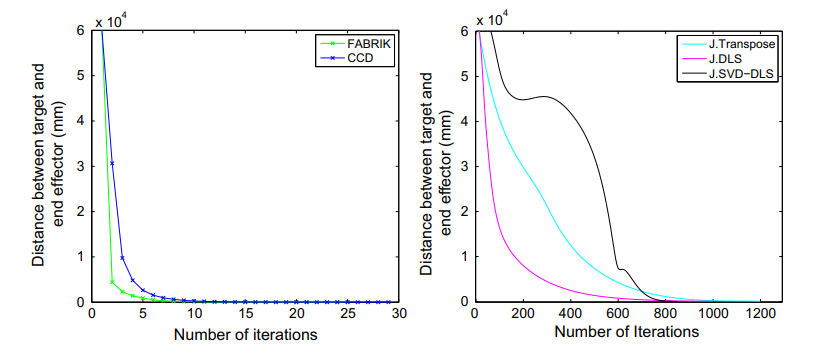
\includegraphics[width=0.95\linewidth]{Figures/FABRIKComparisons}
    \caption{FABRIK approaches an error of zero faster than other iterative methods \cite{fabrik2011}}
    \label{fig:IterativeComparisons}
\end{figure}

FABRIK is relatively simple to implement. It starts from the last link, and adjusts it so the end effector is at the final goal position, and points it toward the joint it should be connected to. Then, the same thing happens to the next link: it moves so one end connects to the last link, and then points toward the joint it should be connected to. This happens all the way up the link from end to the starting joint, and then back again to the end effector to form one iteration, as shown in Figure \ref{fig:FABRIKSteps}. Since computation is based on basic geometry, FABRIK is simple to implement and fast to compute.

\begin{figure}[thbp]
    \centering
    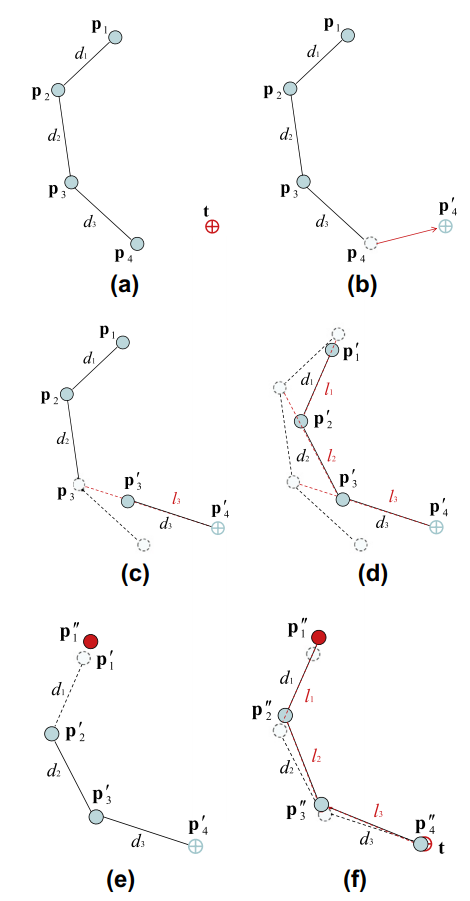
\includegraphics[width=0.85\linewidth]{Figures/FABRIK.png}
    \caption{Steps to Approximate Inverse Kinematics using FABRIK \cite{fabrik2011}}
    \label{fig:FABRIKSteps}
\end{figure}

However, the best part of FABRIK is its versatility. It has proven itself to be resistant to singularities, as well as work with multiple end effectors. \cite{fabrik2011}. It also works with joint limits, and can even act as a closed loop controller when implemented correctly. Better yet, there hasn't been a case where FABRIK has shown no weakness, and is faster than all other known methods.

\subsection{Dynamic Walking}
One very effective method to designing a walking gait is to look toward nature for inspiration. There are two concepts that can be used on legged robots that come from animals: central pattern generators and reflexes/responses
\subsubsection*{Central Pattern Generators}
A Central Pattern Generator (CPG) is a control method that generates trajectories based on loosed-coupled oscillators, similar to the neural circuits found in animals. Essentially, CPGs are a biological neural network that creates a rhythmic output patter without any necessary sensory input. This allows animals to perform basic tasks, like breathe, walk, and chew, and the same basic concept can be used to generate trajectories for robots. There are many ways to create this output, but two of the main methods include the Rulkov map type neuron - which models natural CPGs - and the Kuramoto oscillators - which are more predictable due to their consistent wave. These signals can input into a walking gait to control speed and position of limbs, similar to how a musician would be signaled by different notes in an orchestra. Although CPGs are, by definition, open loop, sensory feedback can be incorporated to modify parameters. This can be used to make changes to the main gait in response to an environment change or possibly a gradual change into another gait.

\subsubsection*{Reflexes \& Responses}
The concept of reflexes and responses is similar to animals. Reflexes are immediate actions to emergency situations. For example, if an unexpected force would push a robot sideways, a reflex would kick out the legs to one side to catch its fall and ensure it doesn't fall over. On the other hand, responses are a change to a gait caused by a change in the environment. An example of a response would be changing the walking gait by some factor when walking on an incline.

\subsubsection*{The Wide Stability Margin}
One way to measure stability of a legged robot is to use the Wide Stability Margin (WSM). It uses the basic physics concept of fulcrums, which states that balance is based on keeping the center of gravity between your points of contact. Finding the WSM is rather straight forward: project the points of contact on the ground. These 4 points, in the case of a quadruped, will draw out a 4-sided polygon. If the projected center of gravity is outside this polygon, then the robot is going to tip over. The Wide Stability Margin is the distance to the closest side of the polygon, and measures how close the robot is to tipping over, as seen in Figure \ref{fig:WSM}. \cite{kimura2007adaptive}

\begin{figure}[thbp]
    \centering
    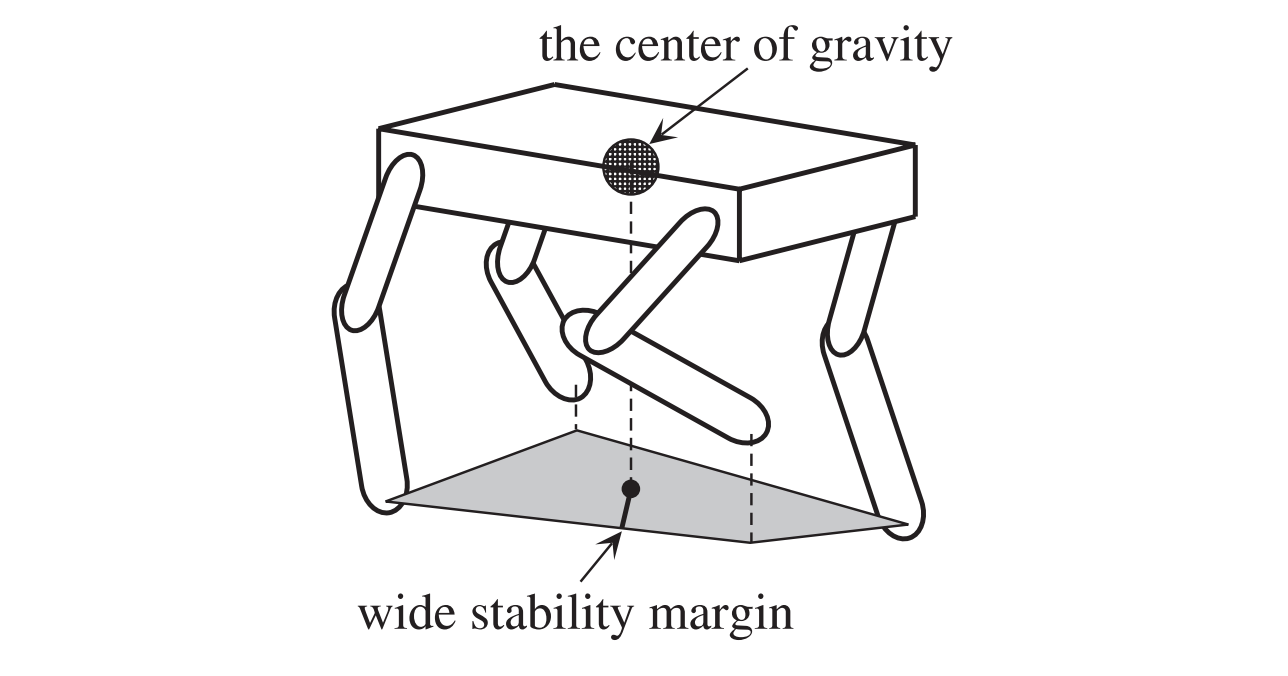
\includegraphics[width=0.95\linewidth]{Figures/WideStabilityMargin.png}
    \caption{Wide Stability Margin on a quadruped \cite{kimura2007adaptive}}
    \label{fig:WSM}
\end{figure}